\documentclass[12pt]{article}

\usepackage{sbc}
\usepackage{graphicx}
\usepackage{url}
\usepackage[T1]{fontenc}
\usepackage[utf8]{inputenc}
\usepackage[brazilian]{babel}
\usepackage{amsmath,amssymb}
\usepackage{booktabs}
\usepackage{microtype}
\usepackage{enumitem}
\usepackage{hyperref}

\setlist{nosep, leftmargin=*}
\setlength{\textfloatsep}{5pt plus 1pt minus 1pt}
\setlength{\floatsep}{5pt plus 1pt minus 1pt}
\setlength{\intextsep}{5pt plus 1pt minus 1pt}
\setlength{\abovecaptionskip}{3pt}
\setlength{\belowcaptionskip}{1pt}
\setlength{\parskip}{2pt}

\makeatletter
\renewcommand\section{\@startsection{section}{1}{\z@}%
                       {-1.8ex \@plus -0.5ex \@minus -0.2ex}%
                       {0.8ex \@plus 0.2ex}%
                       {\reset@font\large\bfseries}}
\renewcommand\subsection{\@startsection{subsection}{2}{\z@}%
                       {-1.4ex \@plus -0.4ex \@minus -0.2ex}%
                       {0.5ex \@plus 0.2ex}%
                       {\reset@font\normalsize\bfseries}}
\makeatother

\hypersetup{
    colorlinks=true,
    linkcolor=blue,
    citecolor=blue,
    urlcolor=blue
}

\sloppy

\title{Análise Experimental de Controle de Congestionamento (TCP CUBIC vs. BBR) e Retomada de Sessão (0-RTT) em Redes Degradadas}

\author{João Marcos Sousa Rufino Leal\inst{1} \and Marcos Willian de Sousa e Silva\inst{1}}

\address{Departamento de Computação -- Universidade Federal do Piauí (UFPI) -- CSHNB -- Picos -- PI\\
  \texttt{jsousarufinoleal@ufpi.edu.br}, \texttt{marcos.sousa@ufpi.edu.br}
  \par\vspace{0.1cm}
  Vídeo explicativo no YouTube (15--25 min): \texttt{[ESPECIFICAR: inserir URL real do vídeo no YouTube]}
}

\begin{document}

\maketitle

\begin{abstract}
Este artigo apresenta uma avaliação experimental de dois mecanismos da camada de transporte com contêineres Docker e emulação via Linux Traffic Control (\texttt{tc netem}): (i) o controle de congestionamento baseado em perda (TCP CUBIC) vs. baseado em modelo de BDP (TCP BBR) em fluxos de 15~s via \texttt{iperf3}; e (ii) o estabelecimento rápido de conexão e retomada de sessão no QUIC (HTTP/3 Cold 1-RTT e Warm/Resumption 0-RTT) frente ao HTTPS/HTTP/2 sobre TCP+TLS~1.3 para um objeto de 1~KB via \texttt{curl}. Os resultados ($N=5$ repetições) mostram que, sob canal WAN degradado (50~ms de RTT e 2\% de perda), a vazão do TCP CUBIC cai para $2{,}63 \pm 0{,}56$~Mbps devido às retrações multiplicativas de \textit{cwnd}, enquanto o TCP BBR mantém $303{,}13 \pm 18{,}87$~Mbps ($115{,}3\times$ maior) ao estimar a banda de gargalo e o RTT mínimo. Em WAN sem perda (50~ms de RTT), o TTFB médio reduziu-se em degraus próximos de 1~RTT ($\approx 51$~ms): de $163{,}57 \pm 2{,}73$~ms no HTTP/2 (3~RTTs) para $112{,}36 \pm 0{,}99$~ms no HTTP/3 Cold (2~RTTs) e $61{,}46 \pm 0{,}95$~ms no HTTP/3 Resumed (1~RTT).
\end{abstract}

\begin{englishabstract}
This paper presents an experimental evaluation of two transport-layer mechanisms using Docker containers and Linux Traffic Control (\texttt{tc netem}): (i) loss-based (TCP CUBIC) vs. BDP model-based (TCP BBR) congestion control over 15~s \texttt{iperf3} flows; and (ii) fast connection establishment and session resumption in QUIC (HTTP/3 Cold 1-RTT and Warm/Resumption 0-RTT) against HTTPS/HTTP/2 over TCP+TLS~1.3 for a 1~KB object via \texttt{curl}. Results ($N=5$ repetitions) show that under a degraded WAN channel (50~ms RTT and 2\% loss), TCP CUBIC throughput drops to $2.63 \pm 0.56$~Mbps due to multiplicative \textit{cwnd} reductions, whereas TCP BBR maintains $303.13 \pm 18.87$~Mbps ($115.3\times$ higher) by estimating bottleneck bandwidth and minimum RTT. In lossless WAN tests (50~ms RTT), mean TTFB decreased in steps close to 1~RTT ($\approx 51$~ms): from $163.57 \pm 2.73$~ms in HTTP/2 (3~RTTs) to $112.36 \pm 0.99$~ms in HTTP/3 Cold (2~RTTs) and $61.46 \pm 0.95$~ms in HTTP/3 Resumed (1~RTT).
\end{englishabstract}

% ==============================================================================
\section{Introdução e objetivos pedagógicos}
% ==============================================================================

O desempenho de aplicações distribuídas depende da capacidade da camada de transporte de utilizar enlaces de longa distância (alto Produto Largura de Banda-Atraso, \textit{Bandwidth-Delay Product}, BDP) e minimizar a latência de estabelecimento de sessões criptográficas seguras \cite{tanenbaum2021}. No protocolo TCP, predominou o controle de congestionamento baseado em perda (\textit{loss-based}), implementado por padrão no Linux pelo algoritmo TCP CUBIC \cite{ha2008cubic}. Contudo, ao interpretar qualquer descarte de pacote como sinal de saturação de buffers nos roteadores, algoritmos baseados em perda degradam a vazão quando submetidos a enlaces com perdas estocásticas não congestionais e tempo de ida e volta (\textit{Round-Trip Time}, RTT) elevado. Para contornar essa limitação, o algoritmo BBR (\textit{Bottleneck Bandwidth and Round-trip propagation time}) \cite{cardwell2017bbr} substitui a heurística de perda por um modelo contínuo da banda de gargalo e do RTT mínimo.

Paralelamente, em transações web curtas, a pilha tradicional HTTPS (HTTP/2 sobre TCP+TLS~1.3) exige múltiplos RTTs em handshakes sequenciais antes que o primeiro byte útil seja transferido \cite{rfc7540,rfc8446}. O protocolo QUIC (base do HTTP/3) \cite{rfc9000,rfc9114} unifica sobre UDP o handshake de transporte e a negociação criptográfica TLS~1.3 em 1-RTT em conexões frias (\textit{Cold}) e permite o envio imediato de dados da aplicação já no primeiro pacote (0-RTT / reaproveitamento de sessão) em reconexões subsequentes (\textit{Session Resumption}).

Dando continuidade direta à bancada experimental em contêineres Docker e emulação via \texttt{tc netem}, este trabalho avalia empiricamente esses dois mecanismos por meio de seis ensaios controlados (E01 a E06) e compara as medições com a fundamentação teórica das Seções 6.5.11, 6.6.1 e 6.6.2 de \cite{tanenbaum2021}.

% ==============================================================================
\section{Fundamentação teórica}
% ==============================================================================

\subsection{Controle baseado em perda (TCP CUBIC) vs. modelo BDP (TCP BBR)}

Em redes com grande BDP, como explica \cite{tanenbaum2021} na Seção 6.5.11 (TCP CUBIC), o crescimento linear do TCP Reno tradicional (1~MSS por RTT) é excessivamente lento para recuperar a capacidade do enlace após uma perda. O TCP CUBIC substitui o incremento linear por uma função cúbica dependente do tempo real $t$ decorrido desde o último evento de perda:
\begin{equation}
W_{\text{cubic}}(t) = C(t - K)^3 + W_{\max}, \quad \text{onde} \quad K = \sqrt[3]{\frac{W_{\max}\beta}{C}}
\label{eq:cubic}
\end{equation}
sendo $W_{\max}$ o tamanho da janela de congestionamento (\textit{cwnd}) no instante do descarte, $C$ uma constante de escala e $\beta \approx 0{,}3$ o fator de decréscimo multiplicativo (contraindo a janela para $cwnd \leftarrow (1 - \beta)W_{\max} = 0{,}7\,W_{\max}$ a cada perda). Embora eficiente em enlaces sem ruído, o CUBIC preserva a premissa de que \textit{perda equivale a congestionamento}. Quando o canal apresenta perdas estocásticas contínuas ($p = 2\%$), o emissor sofre reduções multiplicativas sucessivas de $30\%$ a cada $\approx 1/p = 50$ pacotes enviados. Se o RTT é elevado ($50$~ms), o intervalo entre perdas aleatórias é muito inferior ao tempo $K$ necessário para que $W_{\text{cubic}}(t)$ retorne ao platô $W_{\max}$, o que mantém a janela \textit{cwnd} reduzida durante toda a transmissão.

Já o algoritmo BBR, tratado na Seção 6.6.2 de \cite{tanenbaum2021}, modela o caminho físico como um duto cujo ponto ótimo de operação (ponto de Kleinrock) corresponde ao Produto Largura de Banda-Atraso:
\begin{equation}
\text{BDP} = \widehat{\text{BtlBw}} \times \widehat{\text{RTprop}}
\label{eq:bdp}
\end{equation}
A cada \texttt{ACK} recebido, o BBR atualiza duas estimativas ortogonais: a taxa máxima de entrega recente ($\widehat{\text{BtlBw}} = \max(\Delta \text{entregue}/\Delta t)$) e o menor atraso de ida e volta na janela temporal ($\widehat{\text{RTprop}} = \min(\text{RTT})$). Alternando entre as fases \textit{Startup}, \textit{Drain}, \textit{ProbeBW} e \textit{ProbeRTT}, o BBR regula a taxa de injeção (\textit{pacing rate}) em torno de $\widehat{\text{BtlBw}}$ e limita os dados em voo (\textit{cwnd}) a $\approx 2 \times \text{BDP}$. Assim, o BBR evita \textit{bufferbloat} e não contrai a janela diante de descartes estocásticos isolados, o que preserva a vazão sob 2\% de perda.

\subsection{Handshakes de conexão e retomada de sessão no QUIC (1-RTT vs. 0-RTT)}

Na Seção 6.6.1 de \cite{tanenbaum2021}, mostra-se que o tempo até o início da transferência (\textit{Time to First Byte}, TTFB) de um objeto pequeno depende de quantos RTTs os handshakes de transporte e criptografia exigem antes da entrega do dado útil. No HTTPS / HTTP/2 sobre TCP+TLS~1.3 (E04), as duas camadas operam em sequência: o cliente aguarda 1~RTT para o \textit{3-way handshake} TCP (\texttt{SYN}/\texttt{SYN-ACK}), mais 1~RTT para a negociação criptográfica TLS~1.3 (\texttt{ClientHello}/\texttt{ServerHello}) e outro RTT para enviar o \texttt{GET} e receber o primeiro byte, resultando em $\text{TTFB}_{\text{HTTP/2}} = 2\,\text{RTT}_{\text{hs}} + 1\,\text{RTT}_{\text{req}} + t_{\text{proc}} = 3\,\text{RTT} + t_{\text{proc}}$.

Em conexões frias do HTTP/3 sobre QUIC (E05, Cold 1-RTT), o protocolo incorpora os quadros criptográficos do TLS~1.3 diretamente no pacote UDP \texttt{Initial} \cite{rfc9000,rfc9001}, concluindo transporte e chaves em 1~RTT; com isso, o tempo até o primeiro byte cai para $\text{TTFB}_{\text{H3-Cold}} = 1\,\text{RTT}_{\text{hs}} + 1\,\text{RTT}_{\text{req}} + t_{\text{proc}} = 2\,\text{RTT} + t_{\text{proc}}$. Quando há retomada de sessão (E06, Warm / Session Resumption 0-RTT), requisições subsequentes reutilizam o estado criptográfico ativo e enviam o pedido HTTP/3 sem esperar pelo handshake (0-RTT), reduzindo o total para $\text{TTFB}_{\text{H3-Warm}} = 0\,\text{RTT}_{\text{hs}} + 1\,\text{RTT}_{\text{req}} + t_{\text{proc}} = 1\,\text{RTT} + t_{\text{proc}}$.

% ==============================================================================
\section{Arquitetura do ambiente e metodologia experimental}
% ==============================================================================

A bancada experimental foi orquestrada via \texttt{docker-compose.yml} sobre uma rede bridge isolada (\texttt{net\_bench}, sub-rede \texttt{172.20.0.0/16}), composta por três contêineres com permissão \texttt{cap\_add: [NET\_ADMIN]}:
\begin{itemize}
  \item \textbf{\texttt{server\_tcp\_cc} (\texttt{172.20.0.10}):} Contêiner \texttt{networkstatic/iperf3} em modo servidor (\texttt{-s}) na porta 5201/TCP para os ensaios do Bloco~A.
  \item \textbf{\texttt{server\_http3\_quic} (\texttt{172.20.0.30}):} Contêiner \texttt{caddy:2.7-alpine} com certificados X.509 v3 TLS~1.3 locais (\texttt{/etc/caddy/certs}) servindo um objeto binário determinístico de 1~KB (\texttt{1KB.bin}, 1.024~bytes) em \texttt{/usr/share/caddy} nas portas 443/TCP (HTTP/2) e 443/UDP (HTTP/3 QUIC).
  \item \textbf{\texttt{client\_bench} (\texttt{172.20.0.50}):} Contêiner cliente padronizado (\texttt{curlimages/curl:latest}) equipado com \texttt{iperf3}, \texttt{iproute2} (\texttt{tc}) e o binário \texttt{curl}~8.22 com suporte nativo a HTTP/2 (\texttt{nghttp2}) e HTTP/3 (\texttt{ngtcp2}/\texttt{nghttp3}).
\end{itemize}

O orquestrador automatizado (\texttt{run\_n3.py} / \texttt{run\_n3.sh}) habilita os módulos \texttt{tcp\_cubic} e \texttt{tcp\_bbr} no kernel Linux e aplica as regras \texttt{tc netem} com atraso unidirecional simétrico ($\text{delay} = \text{RTT}/2$) nos três cenários definidos na especificação:
\begin{enumerate}
  \item \textbf{Cenário 1 (LAN, canal ideal):} \texttt{tc qdisc add dev eth0 root netem delay 0.5ms} ($\text{RTT} = 1{,}0$~ms, $0\%$ de perda), aplicado em E01;
  \item \textbf{Cenário 2 (WAN, canal degradado):} \texttt{tc qdisc add dev eth0 root netem delay 25ms loss 2\%} ($\text{RTT} = 50{,}0$~ms, $2\%$ de perda estocástica), aplicado em E02 e E03;
  \item \textbf{Cenário 3 (WAN sem perda, isolamento de handshake):} \texttt{tc qdisc add dev eth0 root netem delay 25ms} ($\text{RTT} = 50{,}0$~ms, $0\%$ de perda), aplicado em E04, E05 e E06.
\end{enumerate}

Cada um dos seis testes foi executado com $N = 5$ repetições independentes. No Bloco~A, o cache de métricas TCP do kernel (\texttt{ip route flush cache}) foi limpo entre cada repetição de 15~s do \texttt{iperf3 -J}. Ao término da bateria, todas as interfaces foram restauradas com \texttt{tc qdisc del dev eth0 root} e os dados brutos foram exportados para \texttt{data/raw/results.csv} e \texttt{results.json}.

% ==============================================================================
\section{Resultados experimentais e discussão}
% ==============================================================================

A Tabela~\ref{tab:resumo_n3} reúne os resultados dos Blocos~A e B ($N=5$ amostras por teste), com médias amostrais ($\bar{x}$), desvios-padrão ($s$), média de retransmissões por fluxo e total acumulado de retransmissões TCP.

\begin{table}[htbp]
\centering
\caption{Resumo dos resultados experimentais (Blocos A e B, $N=5$ repetições por teste).}
\label{tab:resumo_n3}
\resizebox{\textwidth}{!}{%
\begin{tabular}{@{}clllcccc@{}}
\toprule
\textbf{ID} & \textbf{Algoritmo / Modo} & \textbf{Cenário (\texttt{tc netem})} & \textbf{Métrica} & \textbf{Média ($\bar{x}$)} & \textbf{Desv.-padrão ($s$)} & \textbf{Retr./Fluxo} & \textbf{Total Retr.} \\
\midrule
\multicolumn{8}{@{}l}{\textit{\textbf{Bloco A: Impacto do controle de congestionamento (fluxo TCP de 15~s via \texttt{iperf3})}}} \\
\textbf{E01} & TCP CUBIC & LAN (1~ms, 0\% perda) & Vazão (Mbps) & $21.945{,}80$ & $\pm 2.486{,}81$ & $36{,}4 \pm 19{,}8$ & $182$ \\
\textbf{E02} & TCP CUBIC & WAN (50~ms, 2\% perda) & Vazão (Mbps) & $2{,}63$ & $\pm 0{,}56$ & $78{,}0 \pm 4{,}9$ & $390$ \\
\textbf{E03} & TCP BBR & WAN (50~ms, 2\% perda) & Vazão (Mbps) & $303{,}13$ & $\pm 18{,}87$ & $7.819{,}0 \pm 527{,}2$ & $39.095$ \\
\midrule
\multicolumn{8}{@{}l}{\textit{\textbf{Bloco B: Latência de handshake e session resumption (objeto de 1~KB via \texttt{curl})}}} \\
\textbf{E04} & HTTPS (HTTP/2 TCP+TLS) & WAN (50~ms, 0\% perda) & TTFB (ms) & $163{,}57$ & $\pm 2{,}73$ & --- & --- \\
\textbf{E05} & HTTP/3 Cold (1-RTT) & WAN (50~ms, 0\% perda) & TTFB (ms) & $112{,}36$ & $\pm 0{,}99$ & --- & --- \\
\textbf{E06} & HTTP/3 Warm / Resumed & WAN (50~ms, 0\% perda) & TTFB (ms) & $61{,}46$ & $\pm 0{,}95$ & --- & --- \\
\bottomrule
\end{tabular}%
}
\end{table}

\subsection{Análise do Bloco A: TCP CUBIC vs. TCP BBR (Tanenbaum Seções 6.5.11 e 6.6.2)}

A Figura~\ref{fig:bloco_a} apresenta o Gráfico~1 comparando a vazão média e as barras de erro de desvio-padrão dos ensaios E01, E02 e E03. No cenário ideal de rede local (E01: RTT de 1~ms e 0\% de perda), o TCP CUBIC atinge vazão média de $21.945{,}80 \pm 2.486{,}81$~Mbps ($\approx 21{,}95$~Gbps na bridge virtual Docker), valor tomado como referência de capacidade do ambiente.

\begin{figure}[htbp]
\centering
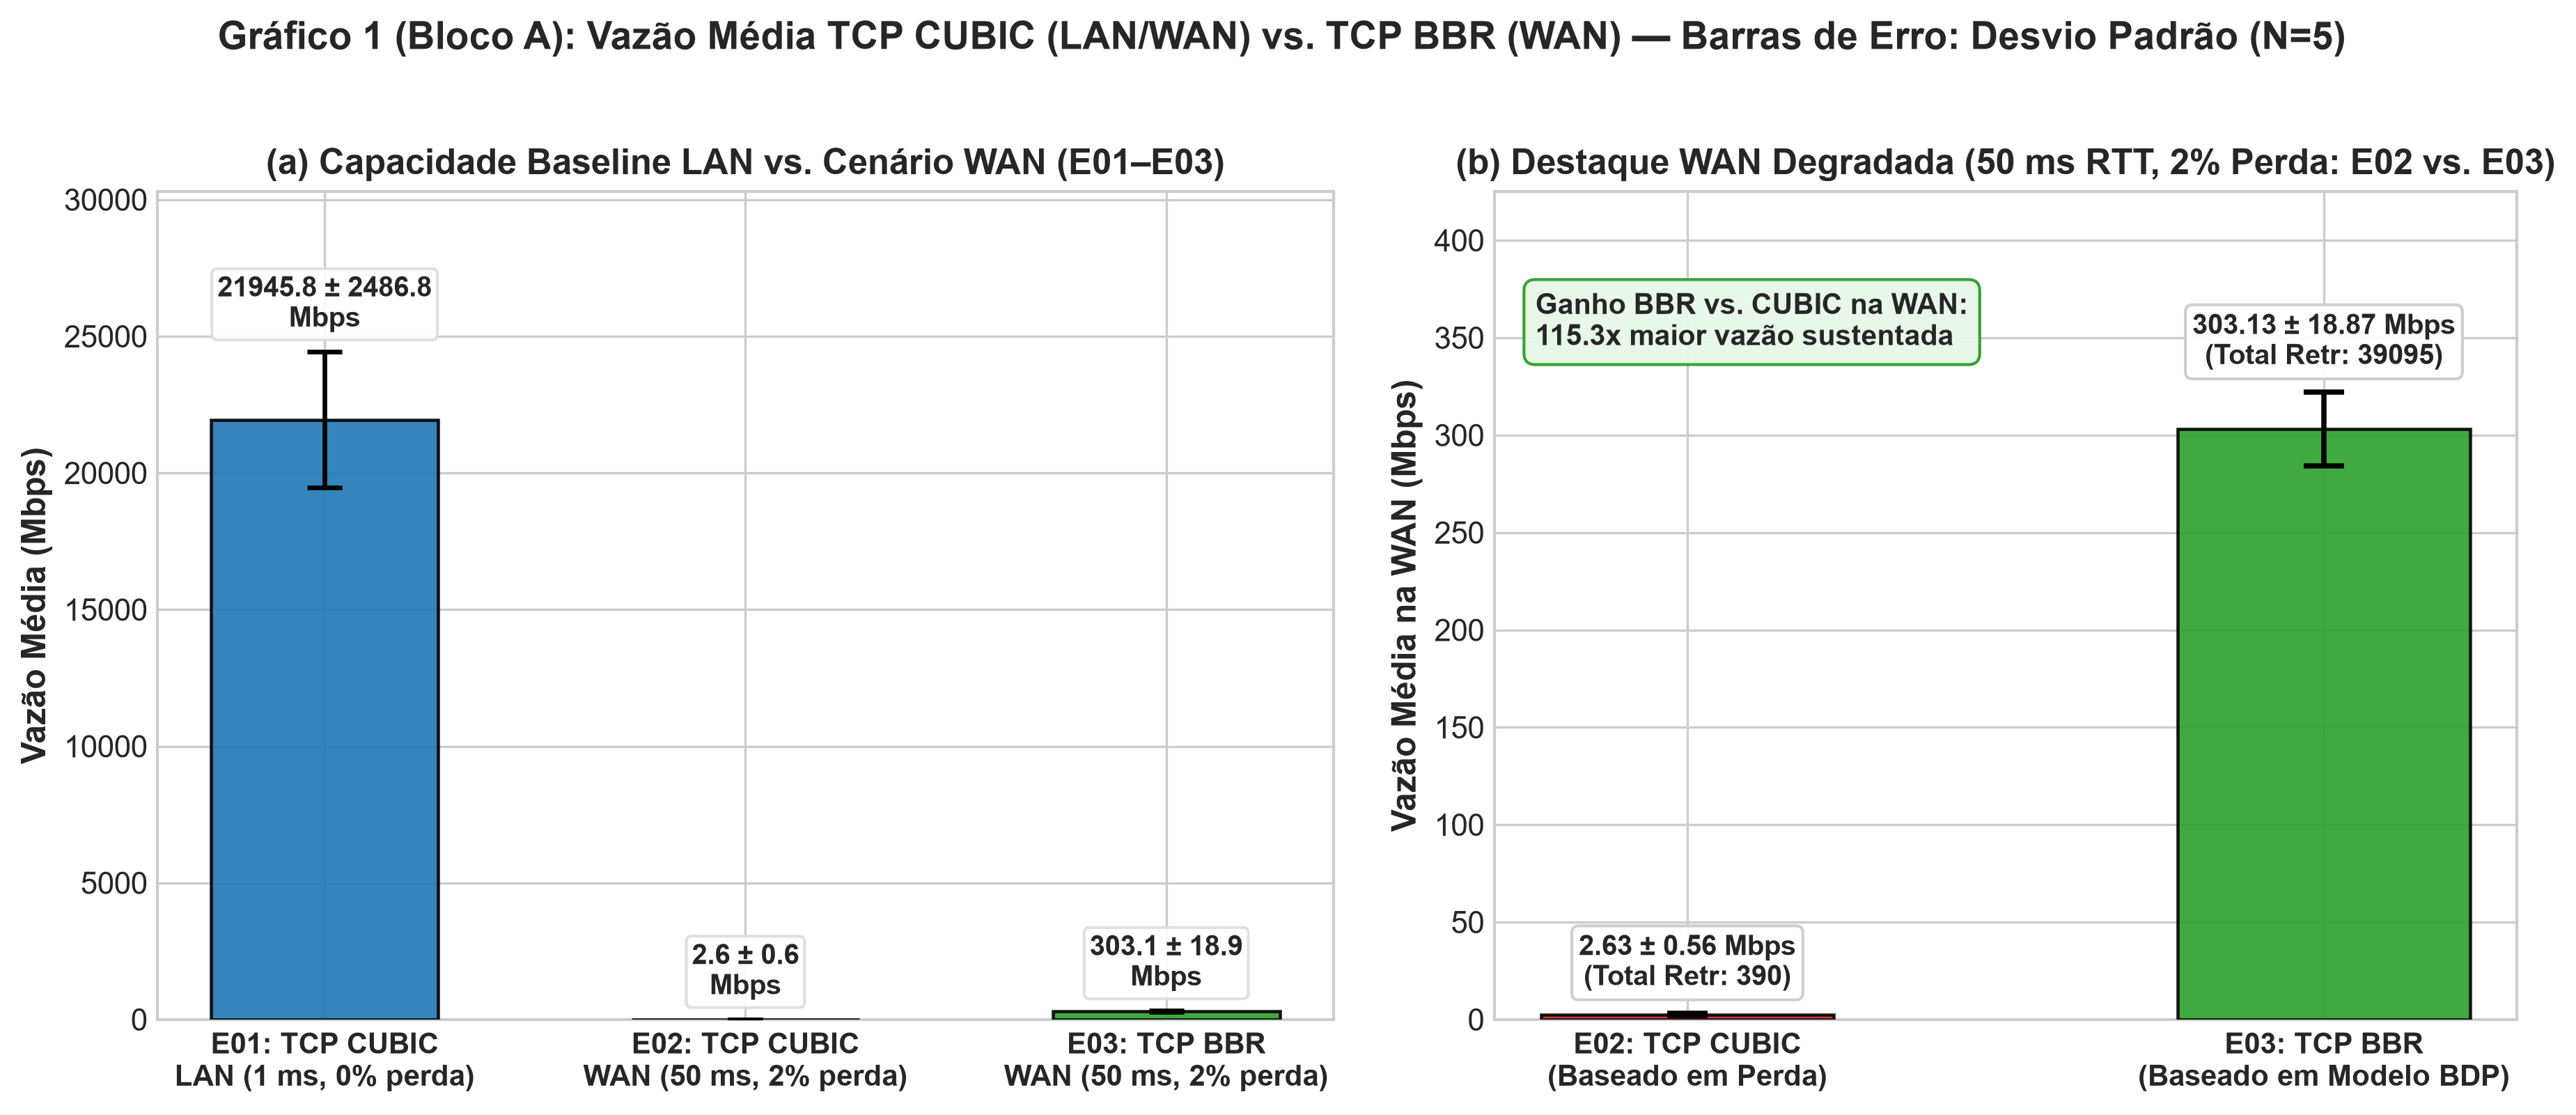
\includegraphics[width=0.84\textwidth]{fig1_bloco_a_vazao_cc.png}
\caption{Gráfico 1 (Bloco A): Vazão média (Mbps) comparando TCP CUBIC (LAN/WAN) e TCP BBR (WAN), com barras de erro representando o desvio-padrão ($N=5$).}
\label{fig:bloco_a}
\end{figure}

Todavia, ao aplicar o cenário WAN degradado com $\text{RTT} = 50$~ms e $2\%$ de perda estocástica (E02), a vazão do TCP CUBIC cai $99{,}99\%$, chegando a $2{,}63 \pm 0{,}56$~Mbps. Conforme a Seção 6.5.11 de \cite{tanenbaum2021}, como o CUBIC interpreta qualquer pacote descartado como congestionamento de fila, cada perda aleatória de 2\% aciona o decréscimo multiplicativo da Equação~\ref{eq:cubic} ($cwnd \leftarrow 0{,}7\,W_{\max}$). Com RTT de 50~ms e probabilidade de perda $p = 0{,}02$, a janela não consegue percorrer a curva cúbica para recuperar o BDP do enlace: os logs JSON do \texttt{iperf3} confirmam que a \textit{cwnd} do CUBIC em E02 permaneceu limitada entre $15$~KB e $36$~KB durante os 15~s, próxima ao limite teórico de fluxos baseados em perda ($\text{Throughput} \approx \frac{\text{MSS}}{\text{RTT}\sqrt{p}} \approx 1{,}65$~Mbps).

Em contraste, quando o algoritmo é alterado para TCP BBR no mesmo canal WAN com 50~ms de RTT e 2\% de perda (E03), a vazão média atinge $303{,}13 \pm 18{,}87$~Mbps, valor 115,3 vezes superior ao do TCP CUBIC (Figura~\ref{fig:bloco_a}b). Conforme descrito na Seção 6.6.2 de \cite{tanenbaum2021}, o BBR não utiliza descartes isolados como sinal para contrair o fluxo; ele estima continuamente a banda de gargalo ($\widehat{\text{BtlBw}}$) e o RTT mínimo ($\widehat{\text{RTprop}} = 50$~ms), mantendo a janela \textit{inflight} dimensionada no Produto Largura de Banda-Atraso (Equação~\ref{eq:bdp}, operando com \textit{cwnd} entre $3$~MB e $7$~MB nos logs do \texttt{iperf3}). A análise do total de retransmissões na Tabela~\ref{tab:resumo_n3} confirma esse mecanismo: no teste E02 (CUBIC), ocorreram apenas $390$ retransmissões totais ($78{,}0/\text{fluxo}$) porque o protocolo ficou limitado e transmitiu apenas $\approx 24{,}7$~MB nos cinco fluxos de 15~s. Já no teste E03 (BBR), o total de $39.095$ retransmissões ($7.819{,}0/\text{fluxo}$) reflete o fato de o BBR ter transferido $\approx 2{,}84$~GB sobre um canal que descarta fisicamente 2\% dos segmentos enviados e retransmitido os pacotes perdidos sem deixar o enlace ocioso.

\subsection{Análise do Bloco B: Handshake e 0-RTT no QUIC (Tanenbaum Seção 6.6.1)}

A Figura~\ref{fig:bloco_b} apresenta o Gráfico~2 com o TTFB médio (\texttt{time\_starttransfer}) e as barras de erro de desvio-padrão para a transferência do objeto de 1~KB sob o Cenário~3 (WAN com $\text{RTT} = 50$~ms e $0\%$ de perda). Sem perda no enlace, o TTFB diminui em degraus próximos aos múltiplos do RTT de 50~ms, de acordo com a Seção 6.6.1 de \cite{tanenbaum2021}:

\begin{figure}[htbp]
\centering
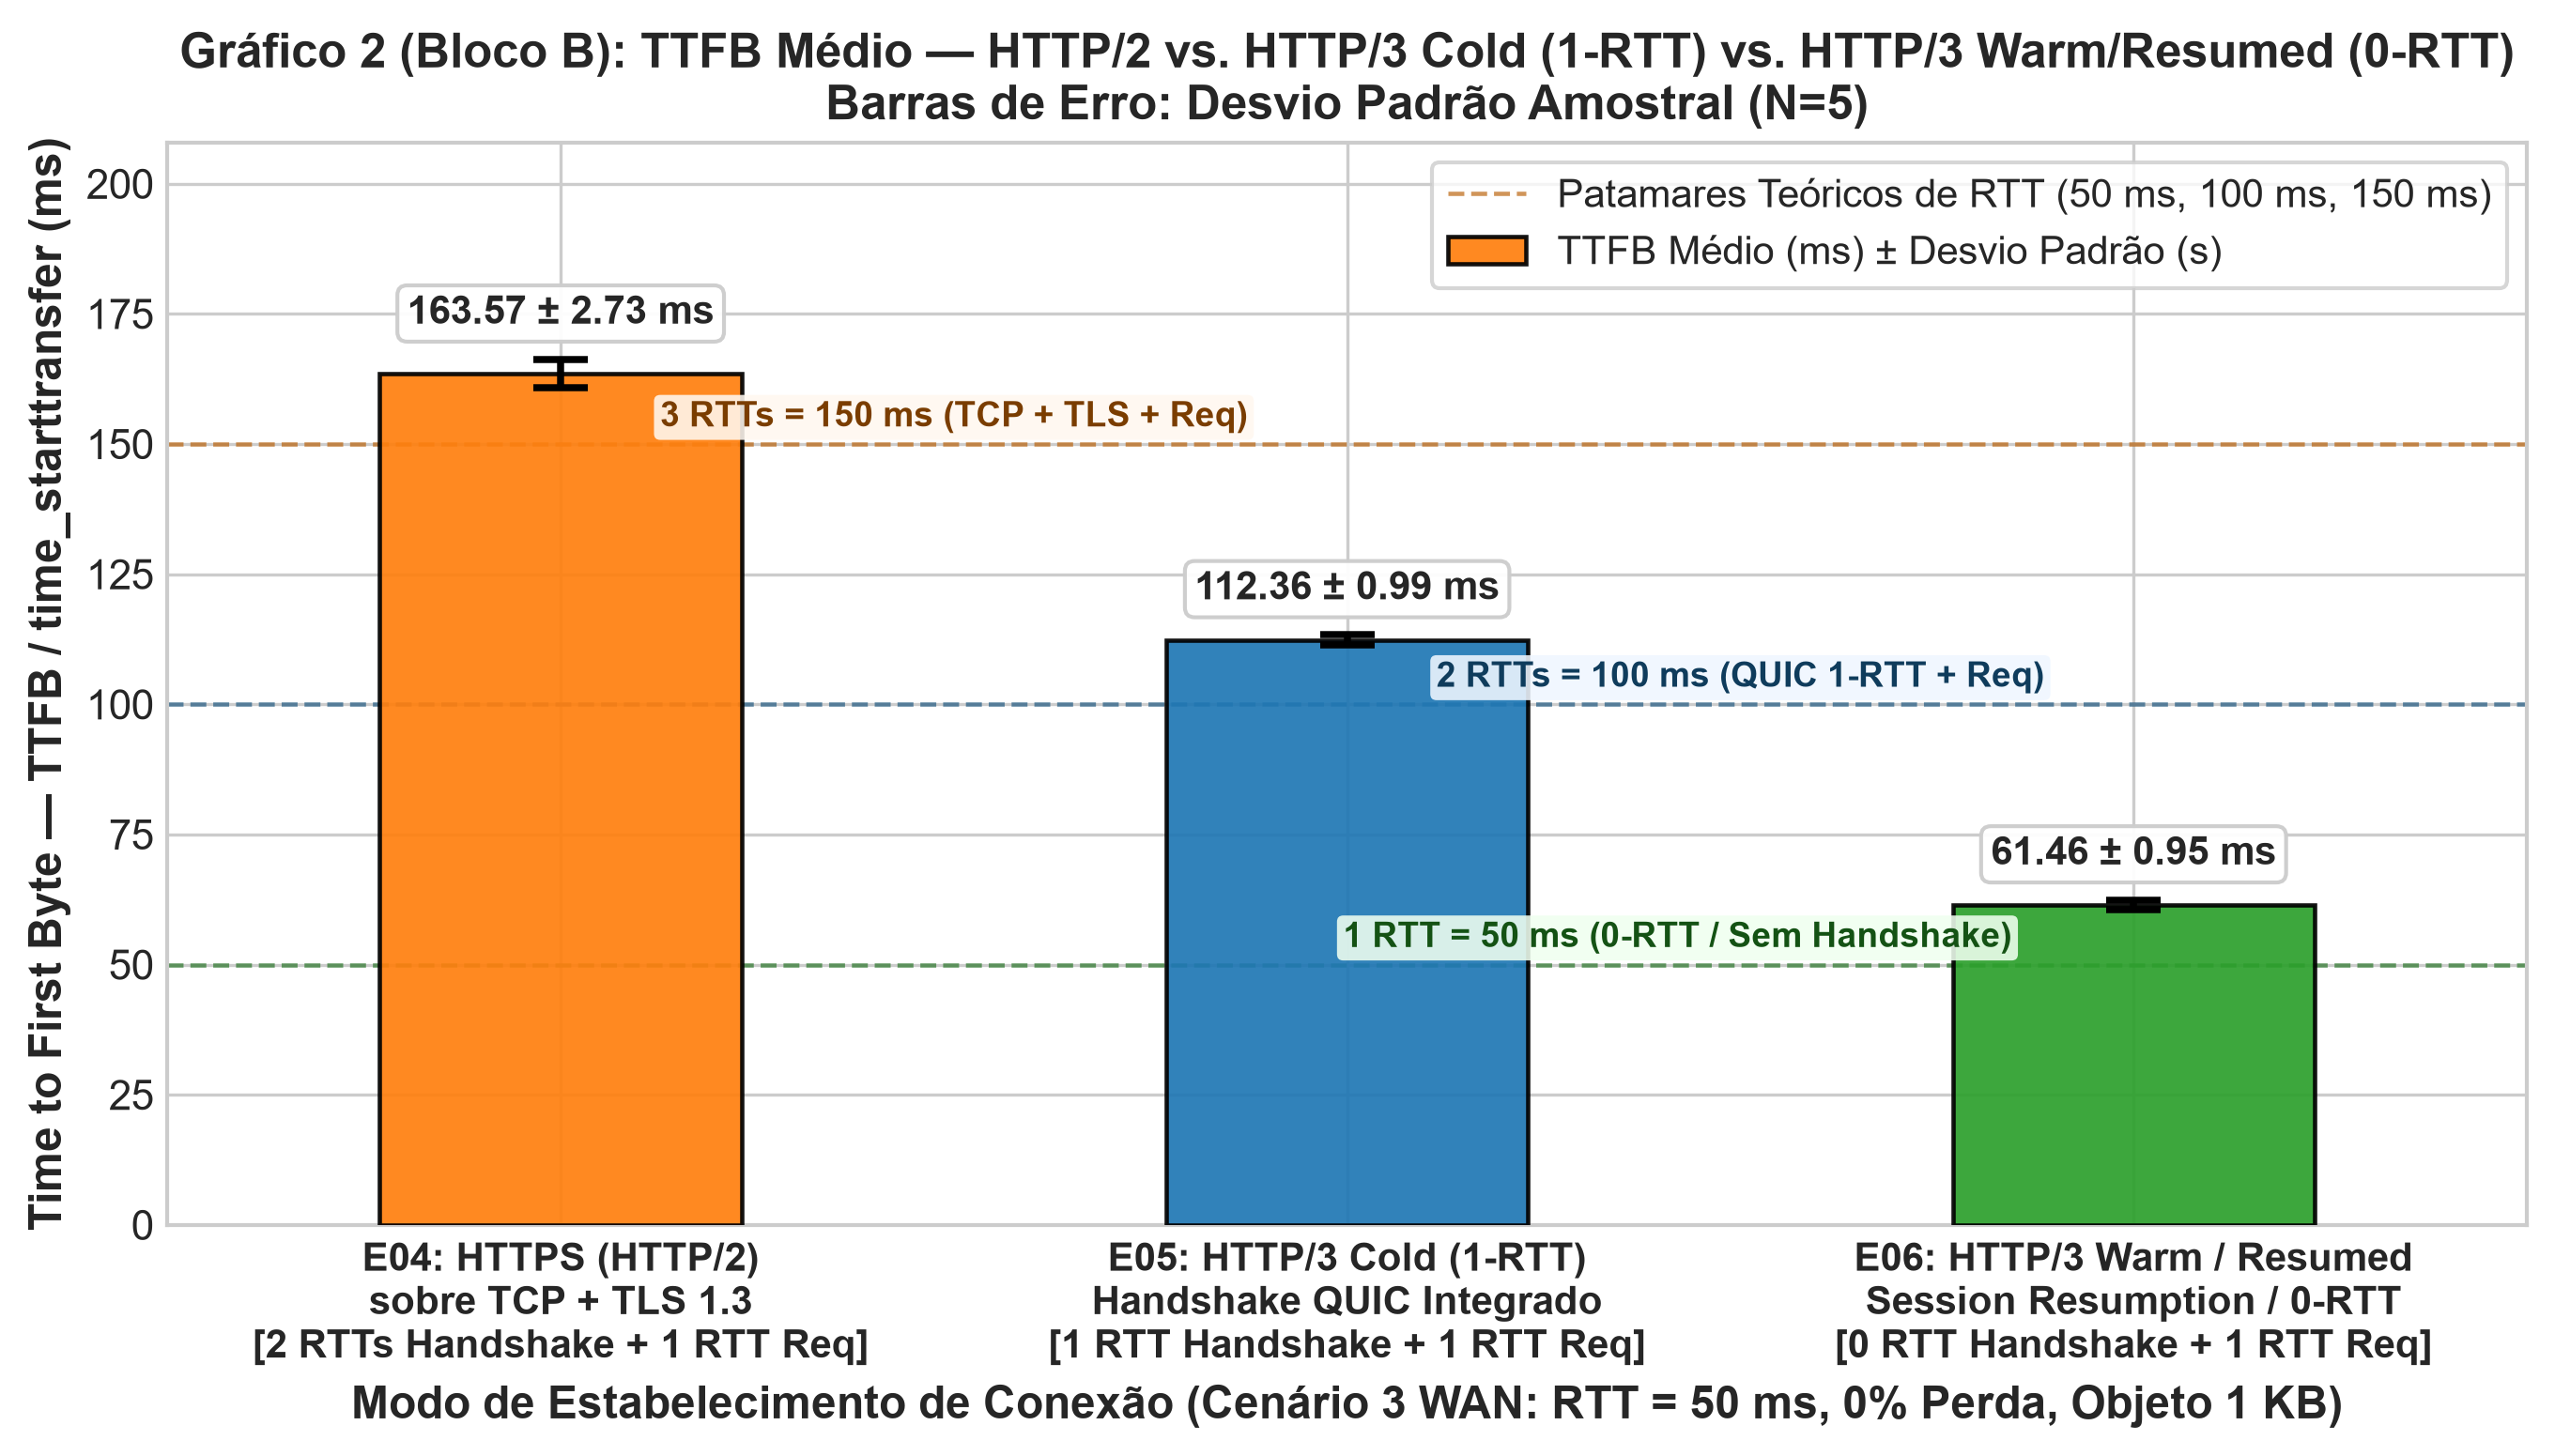
\includegraphics[width=0.60\textwidth]{fig2_bloco_b_ttfb_handshake.png}
\caption{Gráfico 2 (Bloco B): TTFB médio (ms) comparando HTTP/2 vs. HTTP/3 Cold (1-RTT) vs. HTTP/3 Warm/Resumed (0-RTT), com barras de erro de desvio-padrão ($N=5$).}
\label{fig:bloco_b}
\end{figure}

No ensaio E04 (HTTPS / HTTP/2 sobre TCP+TLS~1.3), o TTFB médio foi de $163{,}57 \pm 2{,}73$~ms, valor compatível com os 3~RTTs esperados ($\approx 150$~ms de propagação $+ 13{,}57$~ms de processamento): 1~RTT (50~ms) para o handshake TCP (\texttt{SYN}/\texttt{SYN-ACK}), 1~RTT (50~ms) para o handshake TLS~1.3 e 1~RTT (50~ms) para a requisição \texttt{GET /1KB.bin} e recepção do primeiro byte.

No modo HTTP/3 Cold 1-RTT (E05), o TTFB médio caiu para $112{,}36 \pm 0{,}99$~ms, correspondendo a 2~RTTs ($\approx 100$~ms de propagação $+ 12{,}36$~ms de processamento). Ao integrar o handshake TLS~1.3 no pacote inicial QUIC sobre UDP, o estabelecimento consome 1~RTT, seguido de 1~RTT para a requisição e a resposta; em relação ao HTTP/2 (E04), a redução foi de $\Delta \text{TTFB}_{\text{E04} \to \text{E05}} = 163{,}57 - 112{,}36 = 51{,}21\text{ ms} \approx 1\text{ RTT}$ ($-31{,}3\%$).

Por fim, com retomada de sessão 0-RTT no HTTP/3 Warm (E06), o TTFB médio atingiu $61{,}46 \pm 0{,}95$~ms, equivalente a 1~RTT ($\approx 50$~ms de propagação $+ 11{,}46$~ms de processamento). Com o reaproveitamento da sessão QUIC/TLS (0~RTT de handshake), a redução adicional em relação ao HTTP/3 Cold (E05) foi de $\Delta \text{TTFB}_{\text{E05} \to \text{E06}} = 112{,}36 - 61{,}46 = 50{,}90\text{ ms} \approx 1\text{ RTT}$, o que resulta em redução acumulada de $102{,}11\text{ ms}$ ($\approx 2\text{ RTTs}$, ou $-62{,}4\%$) frente ao HTTP/2 tradicional (E04).

% ==============================================================================
\section{Conclusões}
% ==============================================================================

Os experimentos desta 3ª Avaliação mediram o comportamento dos mecanismos de transporte analisados em cenários WAN. No Bloco~A, verificou-se que a reação baseada em perda do TCP CUBIC (Seção 6.5.11 de \cite{tanenbaum2021}) mantém a janela \textit{cwnd} contraída sob 2\% de perda estocástica ($2{,}63$~Mbps), enquanto o modelo baseado em BDP e RTT mínimo do TCP BBR (Seção 6.6.2 de \cite{tanenbaum2021}) sustenta $303{,}13$~Mbps ($115{,}3\times$ superior). No Bloco~B, observou-se que o handshake integrado do QUIC (Seção 6.6.1 de \cite{tanenbaum2021}) reduz o TTFB em cerca de 1~RTT ($51{,}21$~ms) no modo Cold (1-RTT) e 2~RTTs ($102{,}11$~ms) via retomada de sessão (0-RTT) frente ao HTTP/2 sobre TCP+TLS.

{\small
\bibliographystyle{sbc}
\bibliography{relatorio}
}

\end{document}
